\documentclass[12pt]{article}
\usepackage{verbatim}
\usepackage[dvips]{epsfig}
\usepackage{color}
\usepackage{url}
\usepackage[colorlinks=true]{hyperref}

\begin{document}

\section*{GENESIS: Documentation}

{\bf Related Documentation:}
% start: userdocs-tag-replace-items related-do-nothing
% end: userdocs-tag-replace-items related-do-nothing
{\\\bf Contributed By:}\\
Dave Beeman (dbeeman@dogstar.colorado.edu)\\
Based on {\it fplot.py} for plotting the membrane potential from the G-3 implementation of {\it tutorial4} written by Karthikeyan Subramanian (kartikznov@gmail.com)

\section*{G3Plot (Ver. 0.55)}

This is a preliminary version of a collection of stand-alone Python-based
graphical utilities for plotting the output of GENESIS simulations.  The
simulations use the {\it asc\_file} object to write simulation variables to a
file, with one line per step of the output clock.  These scripts may also
be useful as prototypes of graphical objects that could be more directly
incorporated into the GENESIS GUI \href{../gtube/gtube.tex}{\bf G-Tube}.

These scripts make use of the powerful
scientific graphics capability of \href{http://matplotlib.sourceforge.net/}{\bf Matplotlib}, which easily generates a
wide variety of plots, accompanied by a Navigation Toolbar that allows
for panning and zooming of plots, and saving to publication quality
PNG format images.

To run these scripts, you need Python Ver.\,2.5 or later,
and the {\it Matplotlib} library for Python.  
The installation instructions
explain other requirememts, such as {\it NumPy} (numerical libraries for Python)
that are usually installed along with Python on most Linux systems.

The main script of this package, {\it G3Plot.py}, also requires {\it wxPython}, the
Python implemention of the {\it wxWidgets} widget set now used by GENESIS.

The use of these Python libraries is described in the Frontiers in
Neuroinformatics special issue on \href{http://frontiersin.org/neuroscience/neuroinformatics/specialtopics/8/}{\bf Python\,in\,Neuroscience}.

\subsection*{Python scripts}

Brief description of the scripts and their usage:

\begin{itemize}
\item \href{../g3plot-fplot/g3plot-fplot.tex}{\it fplot.py}\\
Plot files of one ({\it x},{\it y}) pair,
or (time,\,$V_m$) pair per line from a single file given as the argument, e.g.
\begin{verbatim}
   fplot.py Vm.out
\end{verbatim}

\item \href{../g3plot-plotvm/g3plot-plotvm.tex}{\it plotVm.py}\\
An extended version of {\it fplot.py} that uses the {\it Matplotlib}
object-oriented classes, instead of the Matlab-like {\it pylab} commands.  It
takes multiple wildcarded filenames as arguments, and plots them in
different colors on the same axes, e.g.
\begin{verbatim}
   plotVm.py Vm.out pyr4*.out
\end{verbatim}

It has labels and scales specific for membrane potential plots, and is
handy for quickly comparing the results of current injection simulations.
The ({\it x},{\it y}) coordinates of a point on the graph can be displayed in the
Navigation Toolbar by positioning the cursor over it.

\item \href{../g3plot-rasterplot/g3plot-rasterplot.tex}{\it rasterplot.py}\\
Similar to {\it plotVm}, but specialized for creating raster
plots of firing times for a group of neurons.  It takes a single filename
as argument, with a line for each cell containing the spike times separated
by spaces.  The times are plotted as dots with the time on the x-axis and
the cell number (the line number) on the y-axis.

\begin{figure}[h]
  \centering
   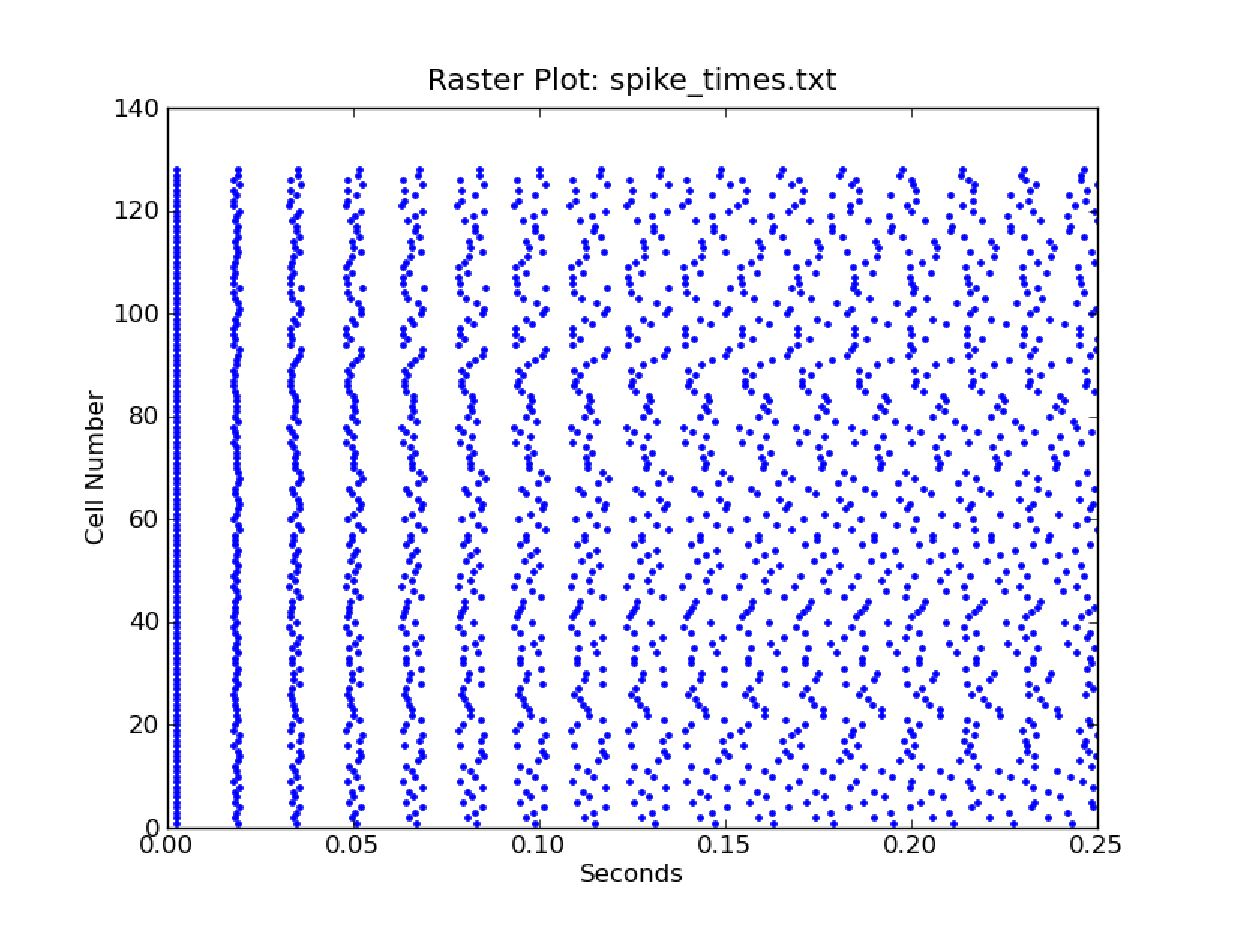
\includegraphics[scale=0.5]{figures/rasterplot.eps}
\caption{\bf G3Plot Raster Plot.}
  \label{fig:g3p-1}
\end{figure}

Figure\,\ref{fig:g3p-1} shows a plot generated with
\begin{verbatim}
   rasterplot.py spike_times.txt
\end{verbatim}

\item \href{../g3plot-g3plot/g3plot-g3plot.tex}{\it G3Plot.py}\\
Enhanced version of {\it plotVm} that wraps {\it Matplotlib}
plots within a {\it wxPython} GUI.  It has several fancy Help menu features
and plotting options to illustrate the
capabilities of {\it wxWidgets} as a GUI for displaying simulation results in
Python.  It can either take the filename list as arguments, or to be
entered in a dialog from the File/Open menu selection.

It addition to the usual Menu bar with File and Help menus, it has a
Control Panel of colored buttons and toggles for clearing the plot,
plotting, setting overlay ON or OFF, and toggling the Legend display.
The Legend identifies each colored line on the graph with the filename in
the same color.

The HTML Usage help describes the use of the {\it Matplotlib} Toolbar that is
used in all these programs, as well as Menu choices and Control Panel
buttons.  The Program Info scrolling message dialog gives information
obtained from program documentation strings about the objects and
functions, and the {\it wxPython} and {\it matplotlib} classes that are used here.

\begin{figure}[h]
  \centering
   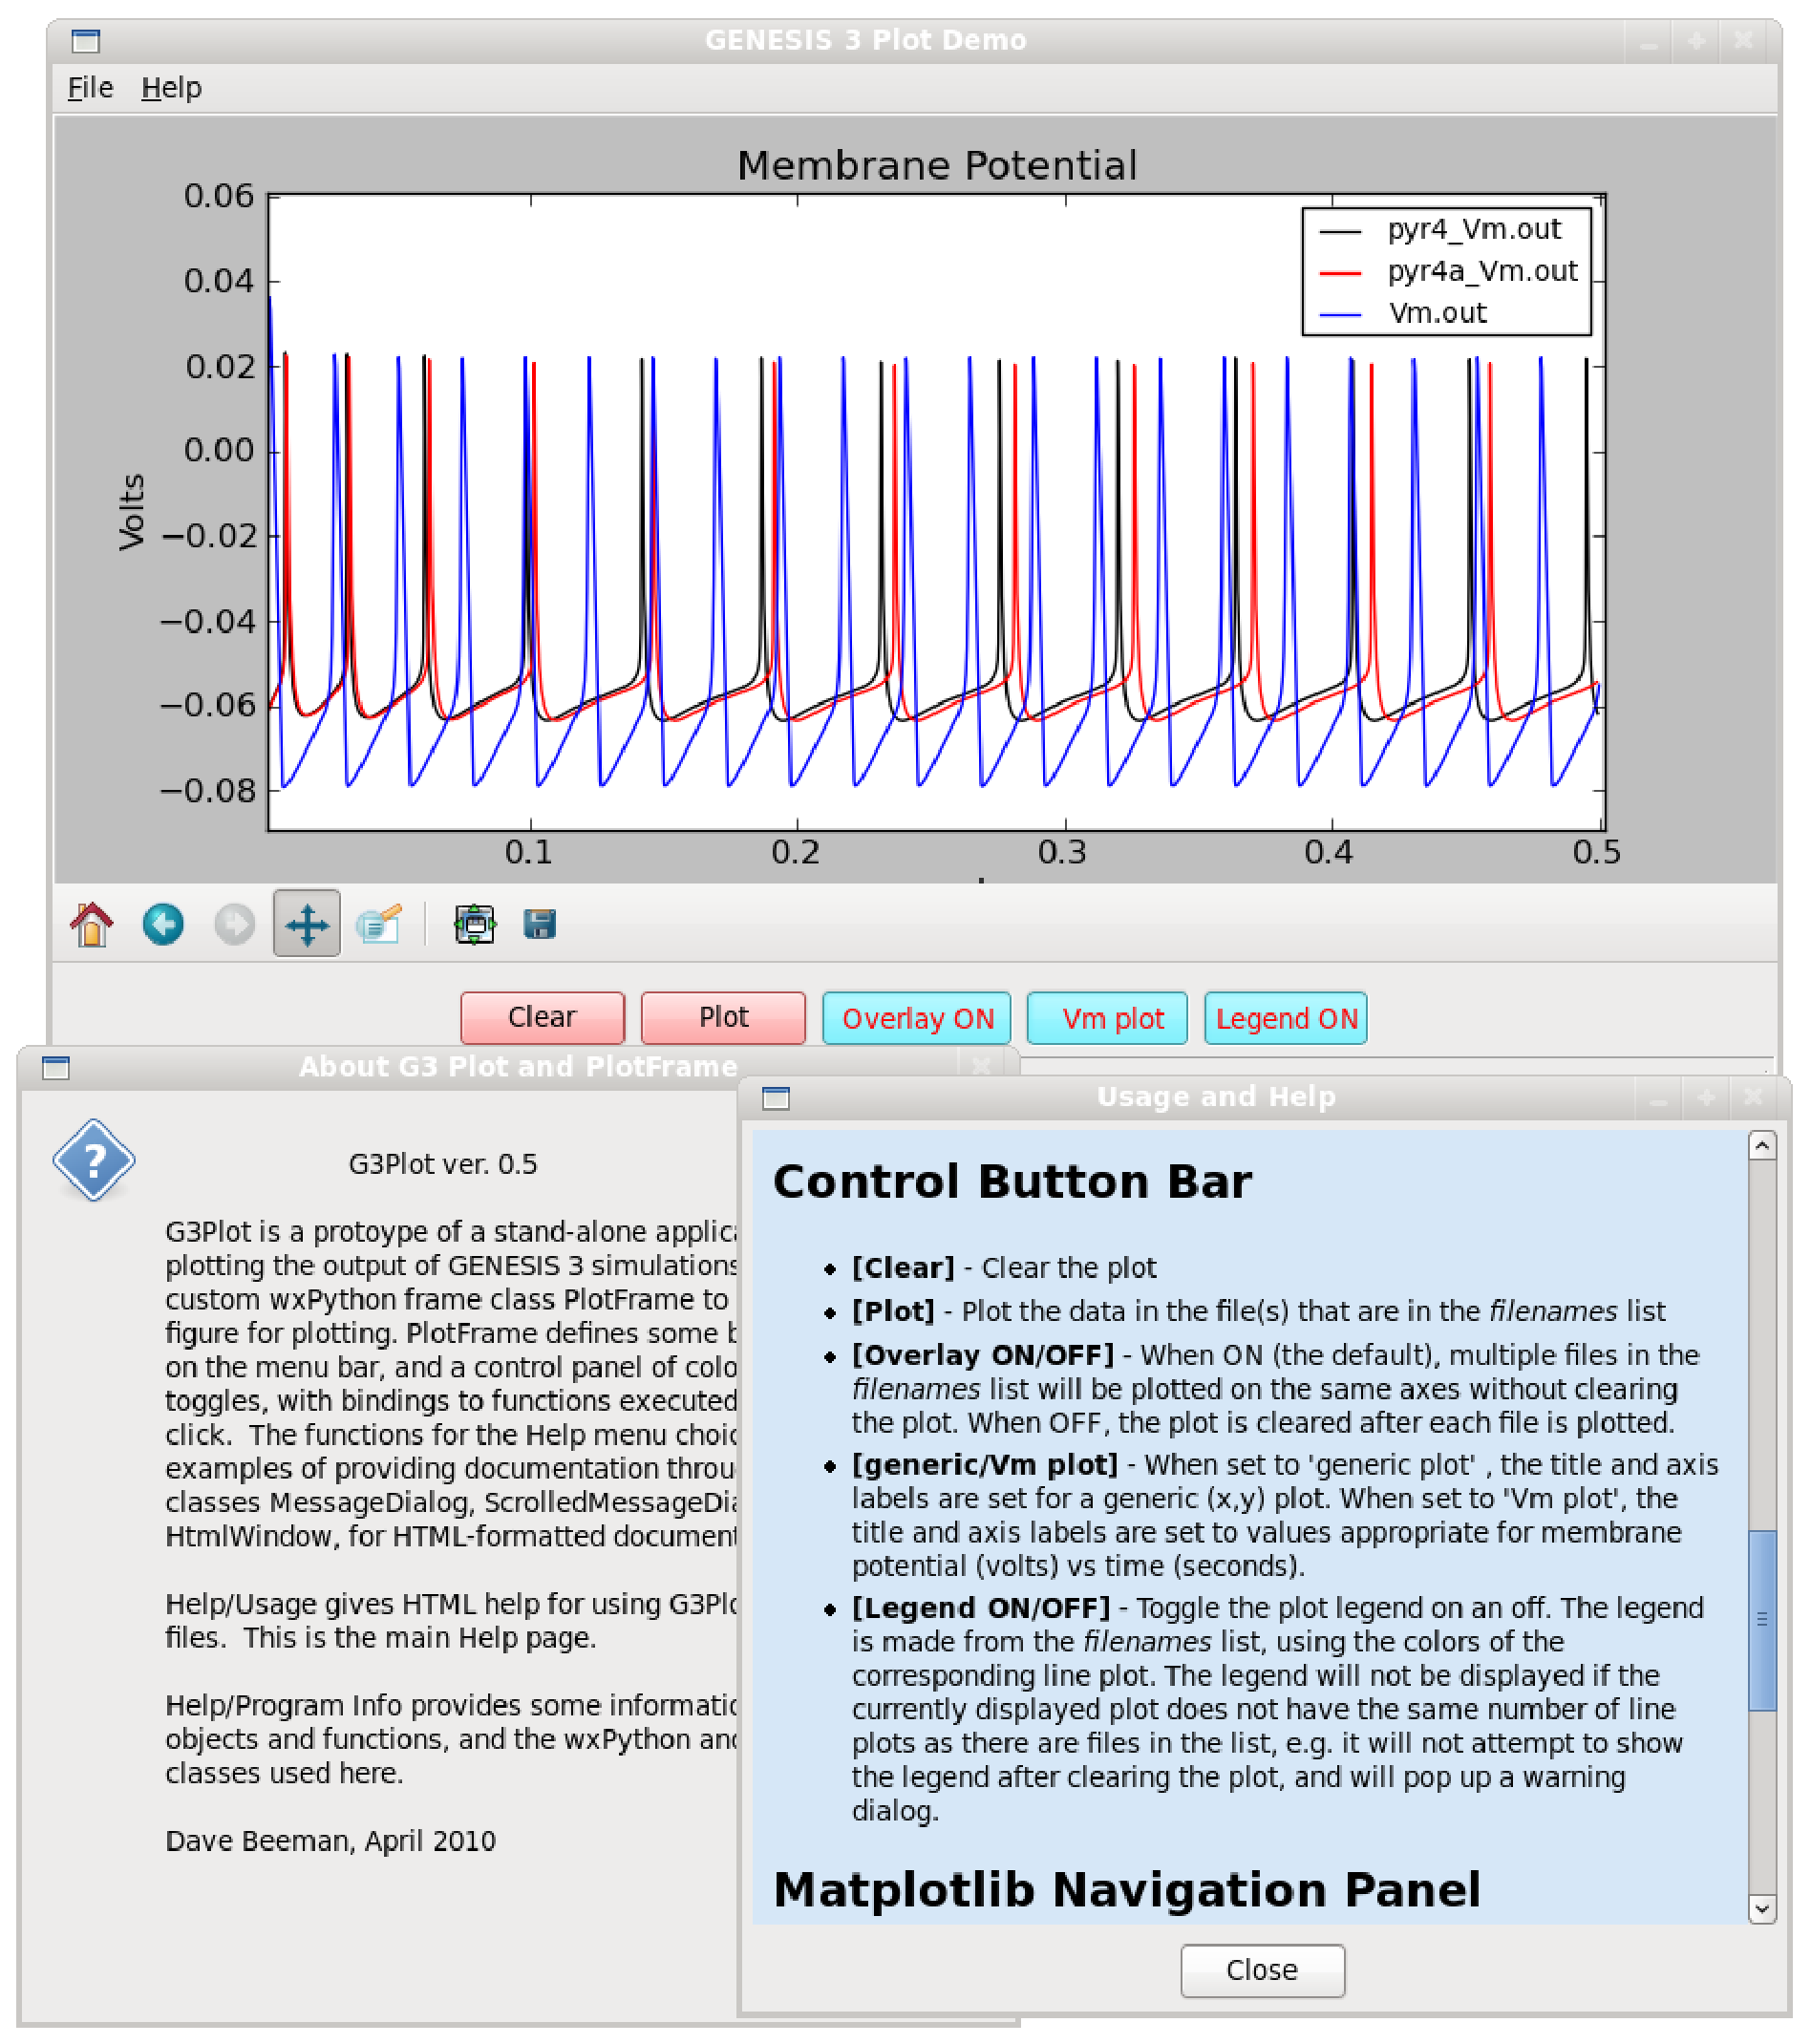
\includegraphics[scale=0.35]{figures/G3Plot-demo.eps}
\caption{{\bf G3Plot GUI:} Includes Usage and About panels.}
  \label{fig:g3p-2}
\end{figure}

Figure\,\ref{fig:g3p-2} shows a screen dump of the GUI with Usage
and About help displayed with the plot.

The screen dump was produced with the following command and arguments:
\begin{verbatim}
   G3Plot.py pyr4*.out Vm.out
\end{verbatim}

\item \href{../g3plot-rowrateplot/g3plot-rowrateplot.tex}{\it rowrateplot.py}\\
This is a utility for analyzing network activity by
displaying a filled contour map of spike frequency vs. simulation time for
groups of neurons.  It takes a single filename as argument, with a line for
each time step containing the simulation time, followed by the average
spike frequency (firing rate) during that time step for each group of
cells.  Typically each cell group is a horizontal row of cells in the
network that are receiving auditory input.  Time is plotted on the x-axis,
cell group (row) on the y-axis, with the average firing frequency of cells
in that row at that time represented by a colored filled contour plot.

\begin{figure}[h]
  \centering
   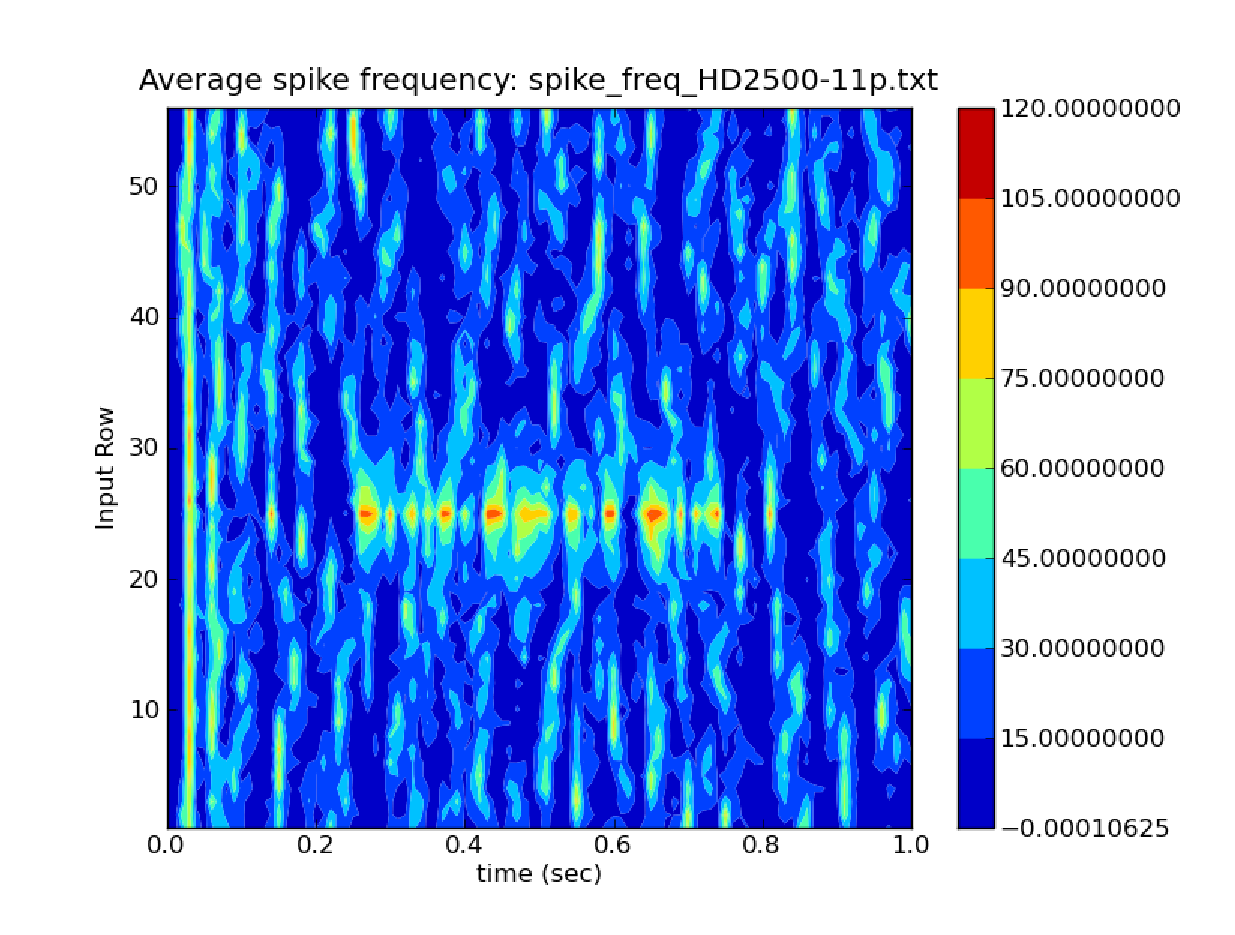
\includegraphics[scale=0.5]{figures/freqplot-HD2500-11p.eps}
\caption{\bf G3Plot Contour Plot.}
  \label{fig:g3p-3}
\end{figure}

Figure\,\ref{fig:g3p-3} (called {\it freqplot-HD2500-11p.eps}) shows the contour plot generated from
\begin{verbatim}
   rowrateplot.py spike_freq_HD2500-11p.txt
\end{verbatim}

The data file was produced from {\it asc\_file} output of a G-2 layer 4
auditory cortex simulation.  The parameters used for the connection weights
in this run provided strong response to the random background input, and to
a 220\,Hz tone pulse with thalamic input to row 25 and nearby rows, lasting
from 0.25--0.75\,s.  {\it rowrateplot.py} will be useful for tuning
parameters to balance excitation and inhibition.

\end{itemize}

\subsection*{Other related files}

\begin{itemize}

\item {\it Vm.out}\\
Typical membrane potential from {\it simplecell} current injection.

\item {{\it pyr4\_Vm.out}, {\it pyr4a\_Vm.out}}\\
Membrane potential from 0.5\,nA injection to
soma of symmetric and asymmetric layer 4 pyramidal cell models.

\item {\it spike\_times.txt}\\
Sample output for a raster plot, produced by {\it raster\_data.g}.

\item{\it raster\_data.g}\\
A G-2 script to generate sample spike time data for
{\it rasterplot.py}. It creates an array of 128 unconnected single compartment
cells based on {\it basic-cell.p}.  The {\it setrandfield} command is used to provide
injection currents randomly distributed within the range 0.27--0.33\,nA.  It uses \href{http://www.genesis-sim.org/GENESIS/Hyperdoc/Manual-19.html}{\bf XODUS}
graphics (which is optional) and some features of the table object
that have not yet been implemented to produce the output file {\it spike\_times.txt}.

\item{\it spike\_freq\_HD2500-11p.txt}\\
Output of network simulation run {\tt HD2500-11p}
    for average spike frequency of each row vs. time.

\item{\bf basic-cell.p} The cell parameter file for the single compartment neuron.

\end{itemize}

\subsection*{BUGS and `features'}

Under Fedora\,12 Linux, the scripts {\it plotVm.py} and {\it rasterplot.py} produce the
warning message:
\begin{verbatim}
/usr/lib64/python2.6/site-packages/matplotlib/backends/backend_gtk.py:621: DeprecationWarning: Use the new widget gtk.Tooltip   self.tooltips = gtk.Tooltips()
\end{verbatim}

{\it G3Plot.py} does not produce this warning, but does not show the ({\it x},{\it y})
coordinates of the cursor in the Navigation Toolbar.  This is a very handy
feature of {\it plotVm.py}, when measuring action potential times and amplitudes.

{\bf Note:} {\it G3Plot.py} uses the {\it Matplotlib} backend API for embedding in {\it wxPython},
{\it matplotlib.backends.backend\_wxagg NavigationToolbar2WxAgg}.  The other
scripts, which do not use {\it wxPython}, use {\it matplotlib.pyplot.figure}, which has
the Toolbar built in.  Possibly, there is a setting to enable this feature
hidden somewhere in {\it NavigationToolbar2WxAgg}.

\bibliographystyle{plain}
\bibliography{../tex/bib/g3-refs.bib}

\end{document}
